\section{Radon in the Shield Cavity}

A potentially dangerous background for XENON100 is the $\gamma$-background from the
decay of ${^{222}}$Rn daughters inside the shield cavity, which has a total volume of 0.58~m$^3$ when the detector is inside.
The average measured radon activity in the LNGS tunnel at the location of the experiment is $\sim$350~Bq/m$^3$ (Figure~\ref{figRadonA}, top). 
Therefore, the shield cavity is constantly purged with high-purity boil-off nitrogen gas when the shield door is closed. Nevertheless, a certain amount of radon can still be present. During the science runs, a low and constant $^{222}$Rn concentration is kept inside the shield.  It is continuously monitored as shown in Figure~\ref{figRadonA}, bottom. The measured values are at the limit of the sensitivity of the radon monitor. No correlation can be seen between the radon concentration inside and outside the shield.

\begin{figure}[!h]
\centering
%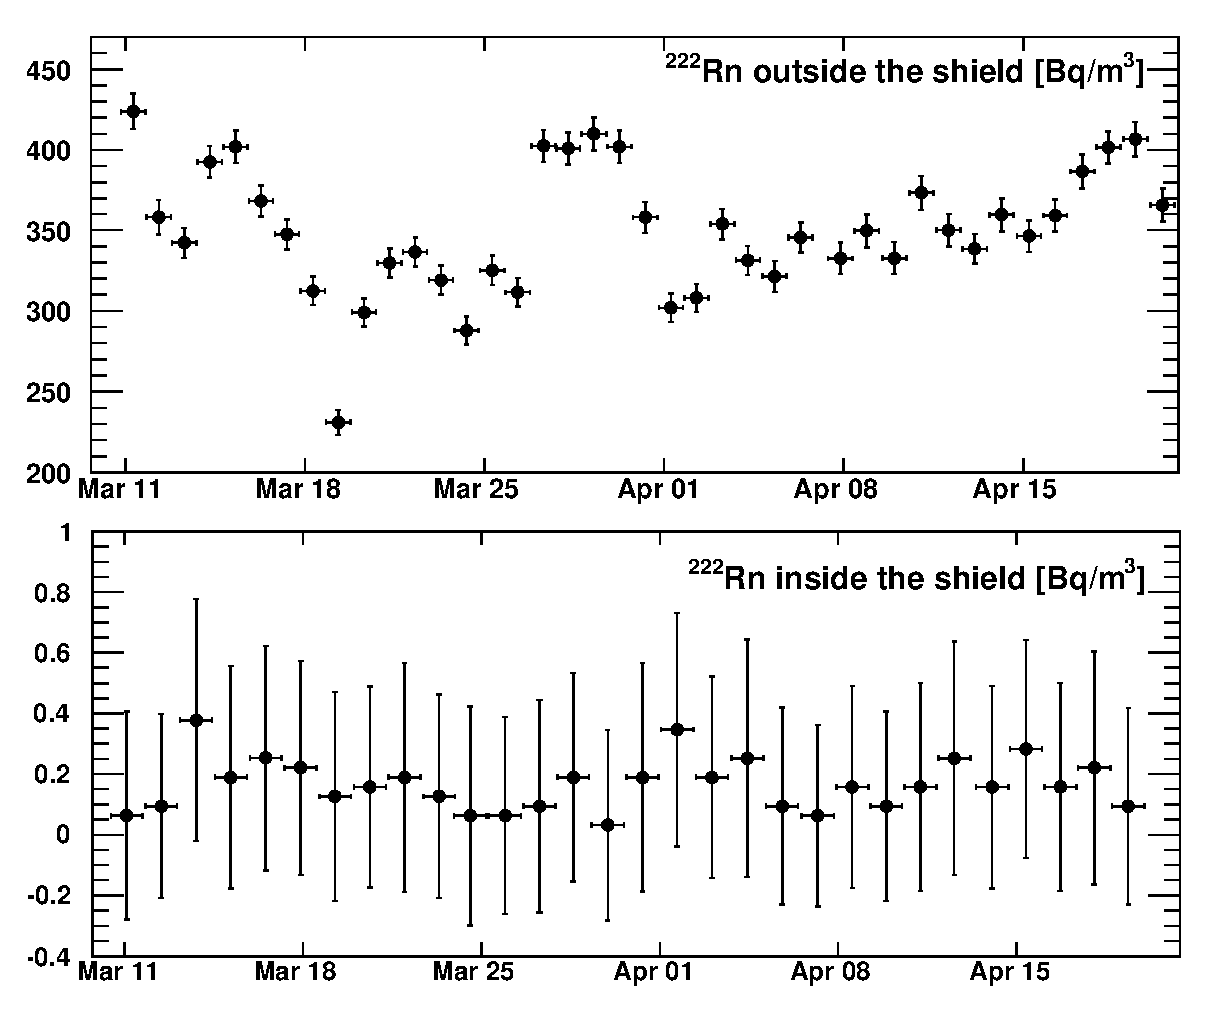
\includegraphics[width=0.5\linewidth]{plots//RnCavity/run08_spring_BoxAndCavity_zoom.eps}
%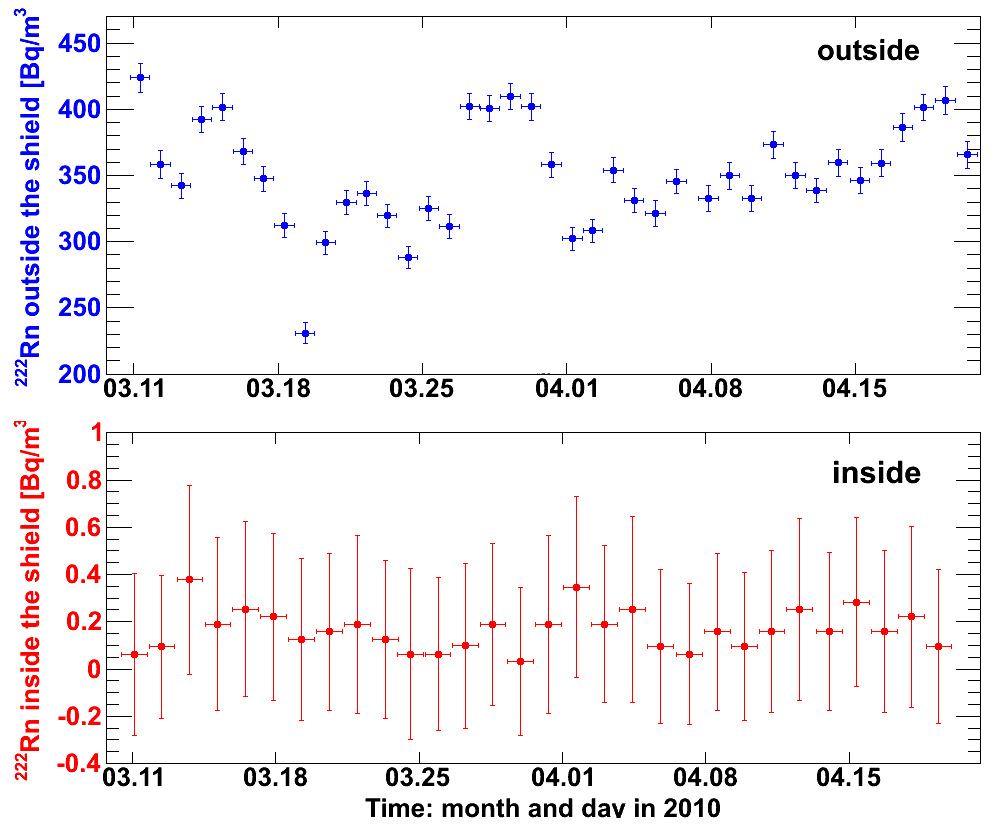
\includegraphics[width=0.5\linewidth]{plots//RnCavity/RnCavity_clr.png}
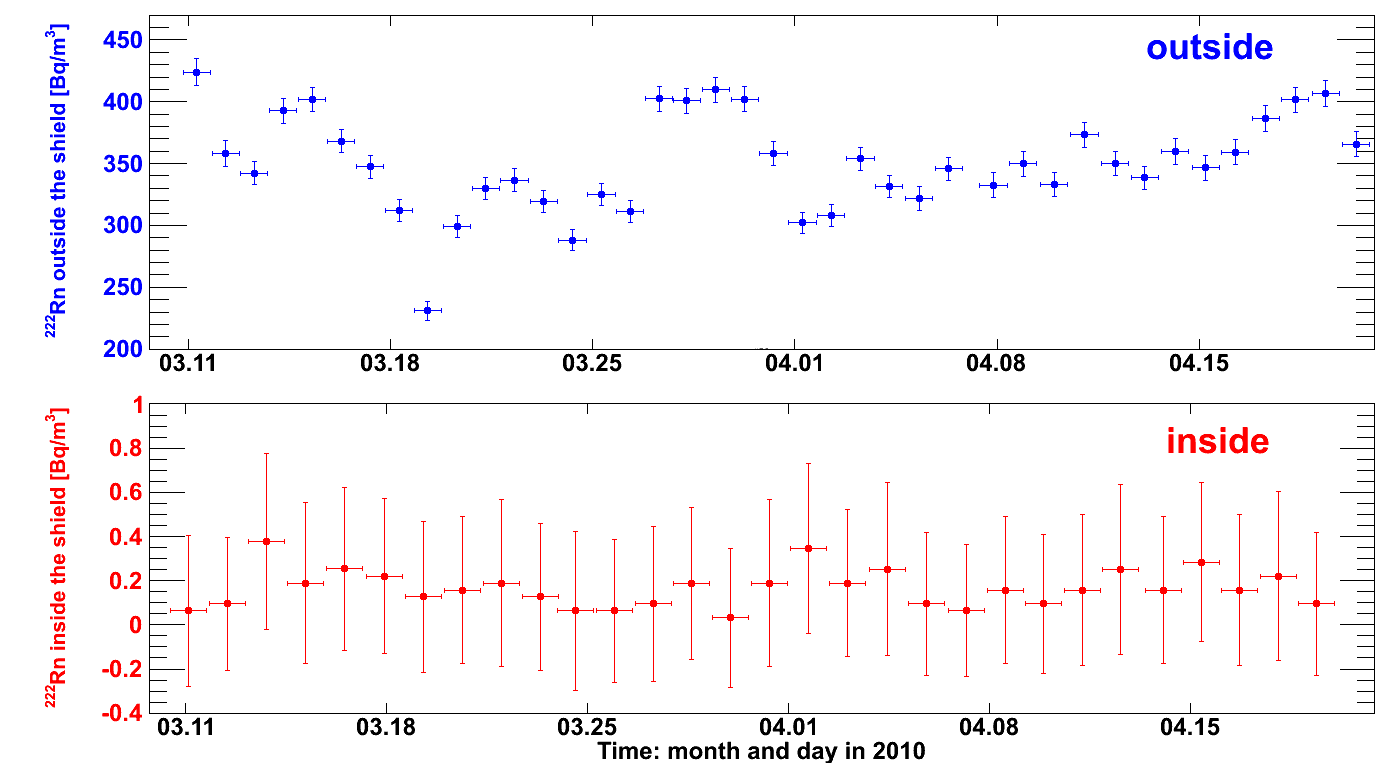
\includegraphics[width=0.9\linewidth]{plots//RnCavity/run08_spring_BoxAndCavity_CLR.png}
\caption[$^{222}$Rn activity measured during 6 weeks of the first science run at the site of the experiment and inside the shield]{$^{222}$Rn activity measured during 6 weeks of the first science run in 2010 (run08 \cite{xe100-run08}), at the site of the experiment (top) and inside the shield (bottom). Each datapoint shows measurements averaged over 24~hours. No correlation can be observed. The measurements inside the cavity are at the sensitivity limit of the radon monitor. }
\label{figRadonA}
\end{figure}

Figure~\ref{figRadonB} shows the predicted background rate from $^{222}$Rn as a function of its concentration inside the shield. Without veto cut, the background rate from 1~Bq/m$^{3}$ of $^{222}$Rn in the shield is 6$\times$10$^{-3}$ events$\cdot$kg$^{-1}\cdot$day$^{-1}\cdot$keV$^{-1}$ in 62~kg target mass, 9$\times$10$^{-4}$ events$\cdot$kg$^{-1}\cdot$day$^{-1}\cdot$keV$^{-1}$ in 40~kg fiducial volume, and 2$\times$10$^{-4}$ events$\cdot$kg$^{-1}\cdot$day$^{-1}\cdot$keV$^{-1}$ in 30~kg fiducial volume. For 30~kg fiducial mass, this is less than 2\% of the background from the detector and shield materials. Additionally, the measured radon concentration is below 1~Bq/m$^{3}$, at the sensitivity limit of the radon monitor.

\begin{figure}[!h]
\centering
\subfigure[]{
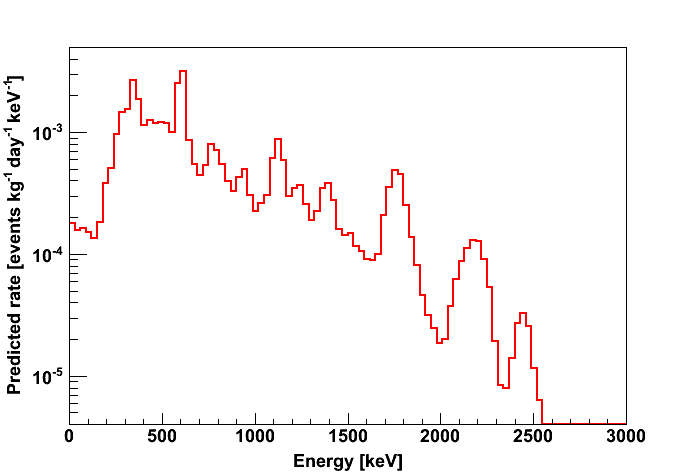
\includegraphics[width=0.475\linewidth]{plots/RnCavity/Rn222_30kg_PassiveVeto.png}
\label{figRadonB_1}}
\subfigure[]{
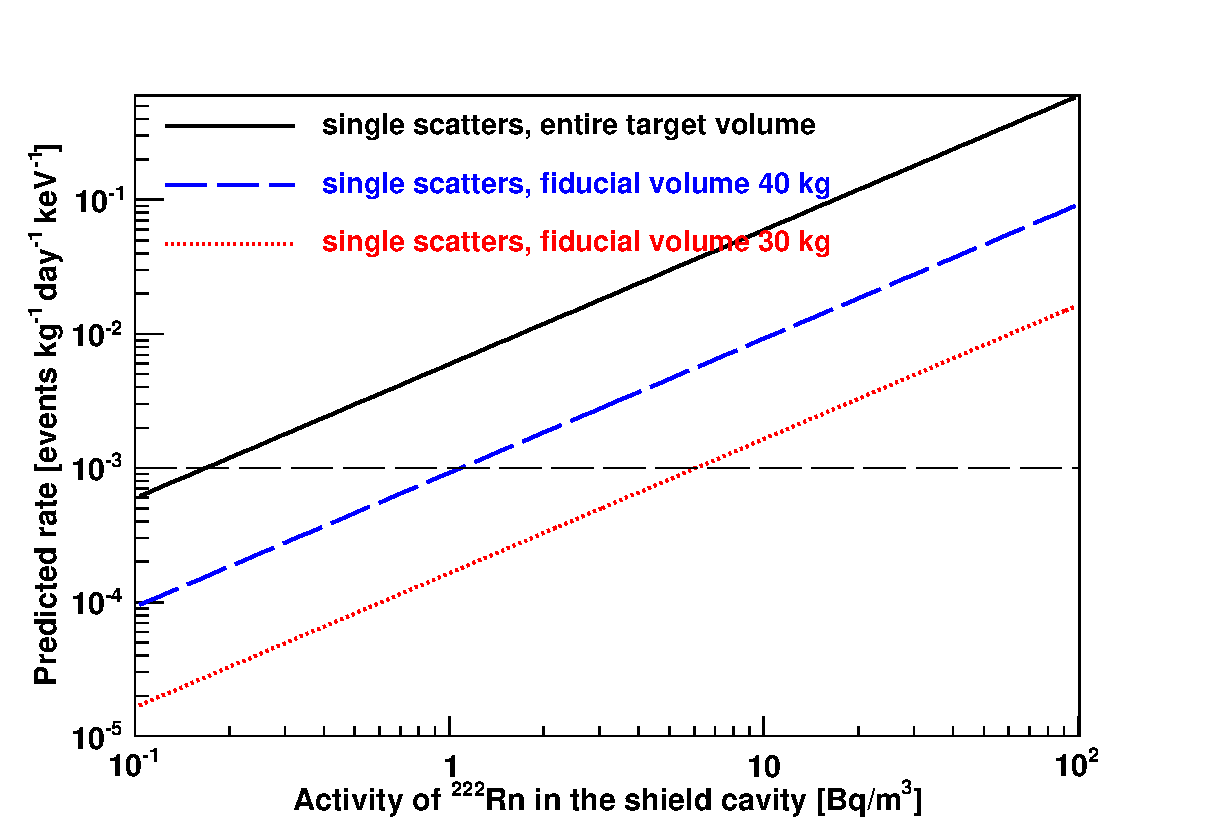
\includegraphics[width=0.475\linewidth]{plots/RnCavity/RnCavity_Rate-vs-Conc_dot.eps}
\label{figRadonB_2}}
\caption[Energy spectrum from 1~Bq/m$^{3}$ of $^{222}$Rn in the shield cavity and predicted rate of single electronic recoils with energy below 100~keV as a function of its concentration]{Energy spectrum in the 30~kg fiducial volume from 1~Bq/m$^{3}$ of $^{222}$Rn in the shield cavity (a) and predicted rate of single electronic recoils with energy below 100~keV as a function of its concentration (b). The simulated energy spectrum has been convoluted with the measured energy resolution. As a reference value, the horizontal dashed line corresponds to a background rate of 10$^{-3}$~events$\cdot$kg$^{-1}\cdot$day$^{-1}\cdot$keV$^{-1}$.}
\label{figRadonB}
\end{figure}
